\section{Phase 3}
In the third phase of this project, our goals were to flesh out pose detection for cars, and add in the ability to detect traffic light colors, and improve the rendering pipeline so that entire scenes could be rendered in a reasonable amount of time.

\subsection{Improved Depth Detection}
Another issue which presented itself in previous phases was the issue with using the centroid of the bounding box for depth estimation. Objects could be occluded in a such a way that the centroid lay on pixels which did not actually belong to the object, and as such the depth would be predicted incorrectly. To solve this, the segementation version of YOLOv9 was used, which provided a mask for each bounding box of a detected object. A simple scheme wherein the median of the depth of each pixel in the mask was used as the depth of the object was implemented. The difference between the outputs of the two network versions, as well as the resulting depth mask, is shown in Figure \ref{fig:depth}.

\begin{figure}
  \centering
  \begin{subfigure}{0.9\linewidth}
    \centering
    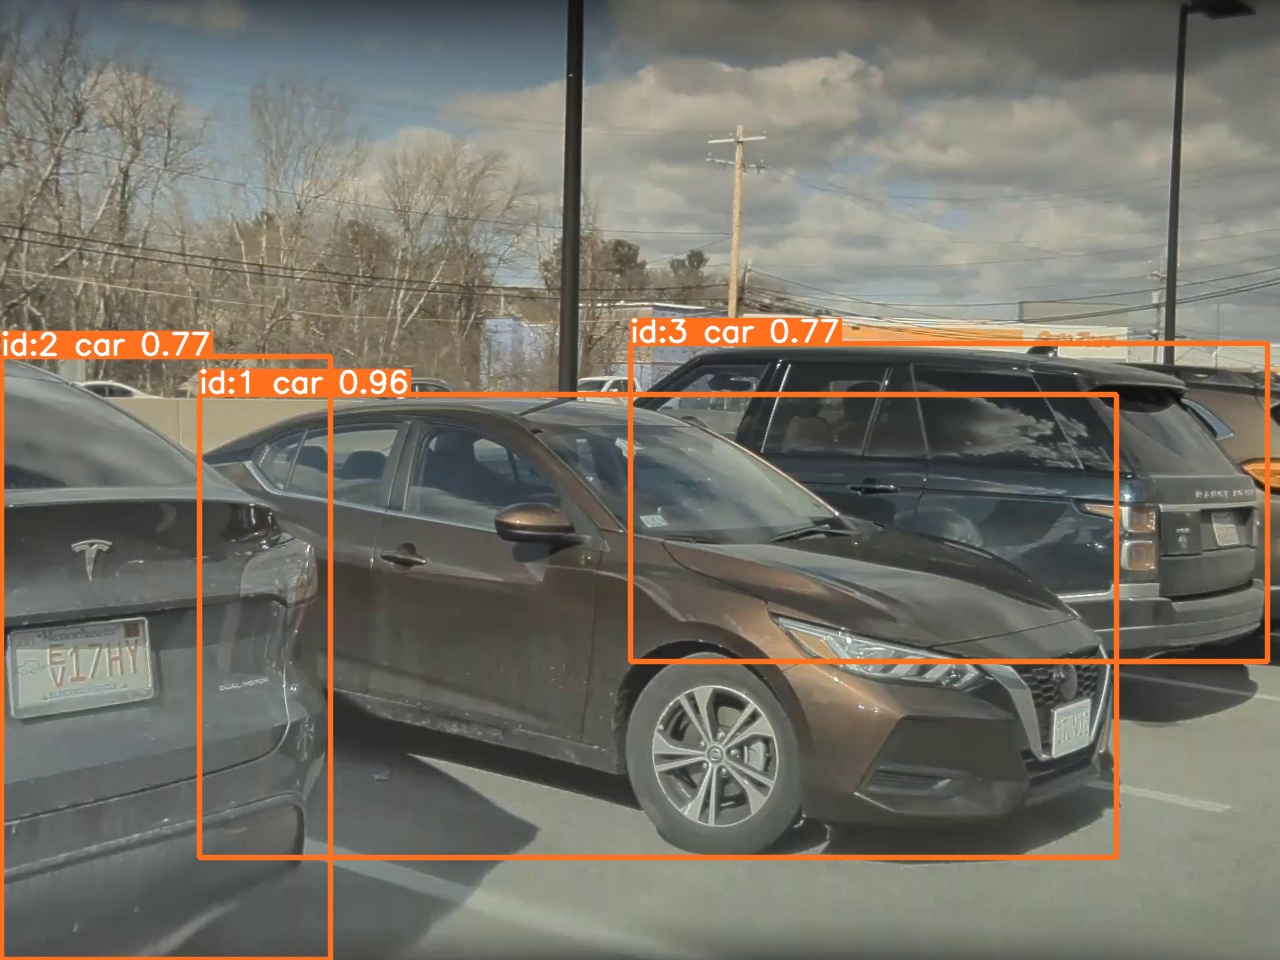
\includegraphics[width=0.95\textwidth]{images/YOLOv9_without_seg.jpg}
    \caption{YOLOv9 without segmentation.}
  \end{subfigure}
  \begin{subfigure}{0.9\linewidth}
    \centering
    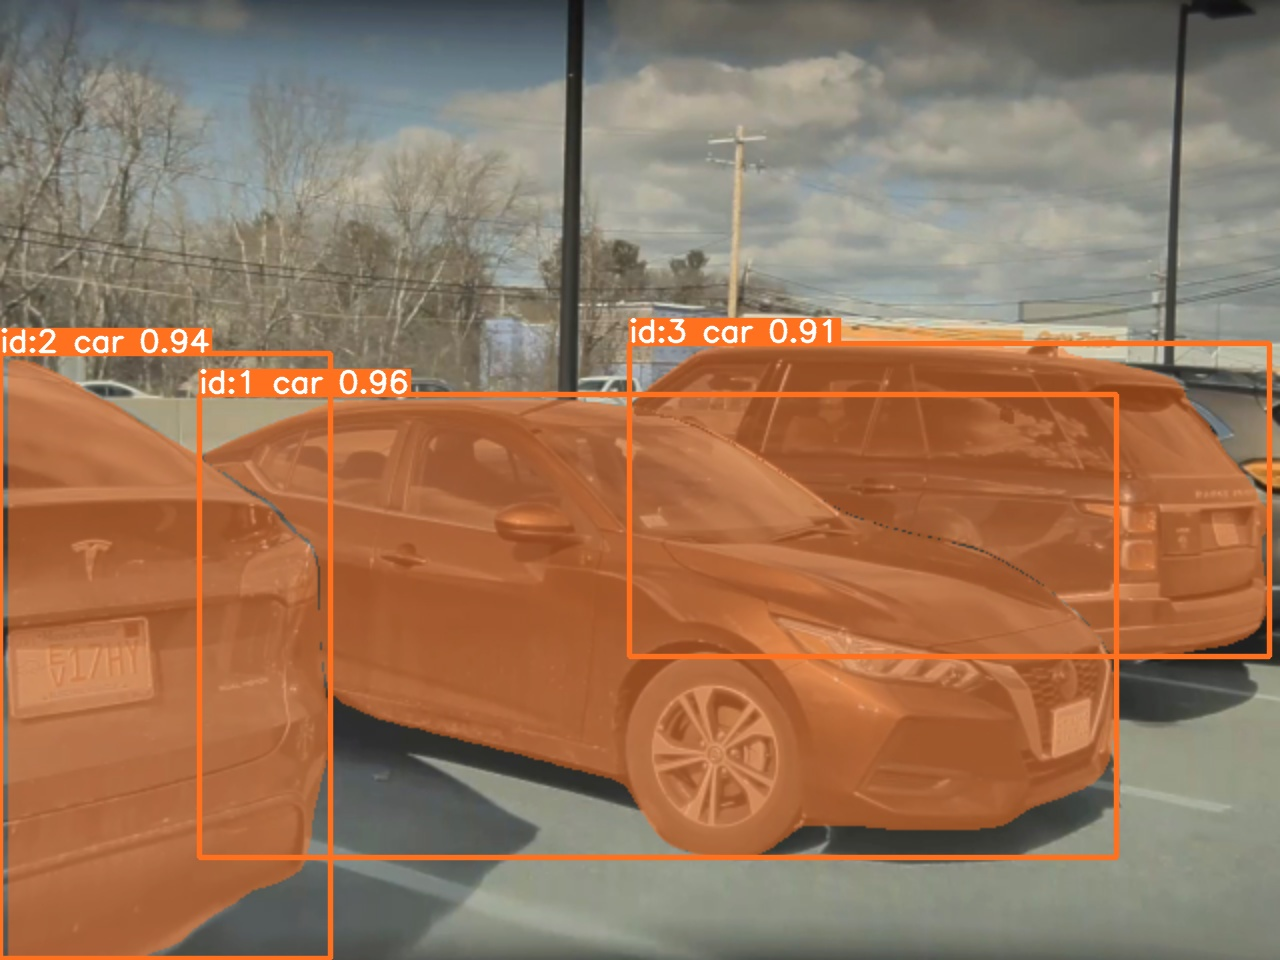
\includegraphics[width=0.95\textwidth]{images/YOLOv9_with_seg.jpg}
    \caption{YOLOv9 with segmentation.}
  \end{subfigure}
  \begin{subfigure}{0.9\linewidth}
    \centering
    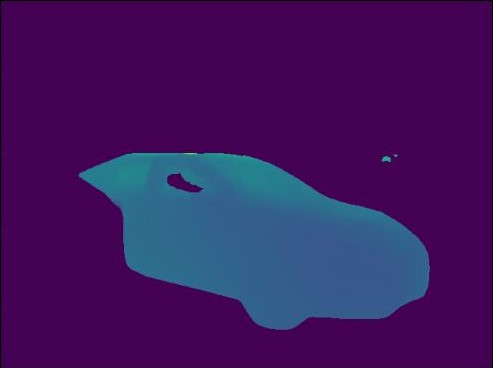
\includegraphics[width=0.95\textwidth]{images/masked_depth.jpg}
    \caption{Masked depth of one car. Notice the outlier points, which are ignored using the median scheme.}
  \end{subfigure}
  \caption{Improved depth detection using segmentation.}
  \label{fig:depth}
\end{figure}

\section{Pedestrian Pose Estimation}
Pedestrian pose estimation was performed using derivative of YOLOv8 trained on poses, povided by ultralytics \cite{YOLOv8Pose}. This network detected pedestrians and accurately predicted poses, but we were unable to integrate it into our pipeline due to time constraints. The output of the network is shown in Figure \ref{fig:pedestrian_pose}.

\begin{figure}
  \centering
  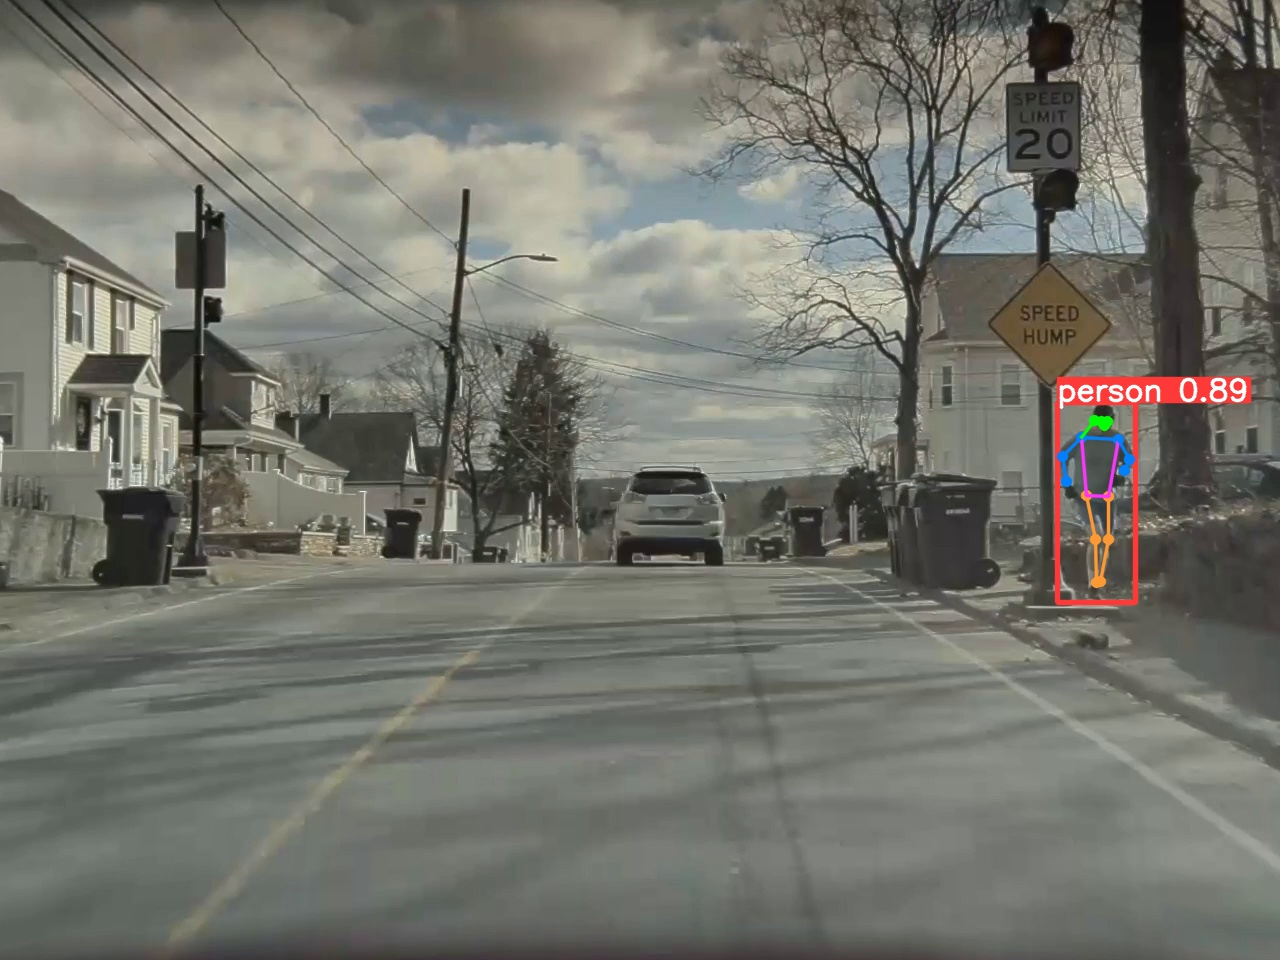
\includegraphics[width=0.95\linewidth]{images/pedestrian_pose.jpg}
  \caption{Pedestrian pose estimation using YOLOv8.}
  \label{fig:pedestrian_pose}
\end{figure}

\section{Shortcomings}
After completing our entire pipeline, there are clearly some shortcomings, and things our team could simply not get working.